% To run the file use one of the following commands
% xelatex  --shell-escape Sample_Poster_EN.tex
%or
% pdflatex  --shell-escape Sample_Poster_EN.tex
\documentclass[a0,portrait]{a0poster}
\usepackage{multicol} % This is so we can have multiple columns of text side-by-side
\columnsep=100pt % This is the amount of white space between the columns in the poster
\columnseprule=3pt % This is the thickness of the black line between the columns in the poster

\usepackage[svgnames]{xcolor} % Specify colors by their 'svgnames', for a full list of all colors available see here: http://www.latextemplates.com/svgnames-colors

\usepackage{times} % Use the times font
%\usepackage{palatino} % Uncomment to use the Palatino font
%\usepackage{subfig}
\usepackage{graphicx} % Required for including images
\graphicspath{{figures/}} % Location of the graphics files
\usepackage{booktabs} % Top and bottom rules for table
\usepackage[font=small,labelfont=bf]{caption} % Required for specifying captions to tables and figures
\usepackage{amsfonts, amsmath, amsthm, amssymb} % For math fonts, symbols and environments
\usepackage{wrapfig} % Allows wrapping text around tables and figures
\usepackage[pages=some]{background}
\backgroundsetup{
scale=1.05,
color=black,
opacity=0.15,
angle=0,
contents={%
  \centering 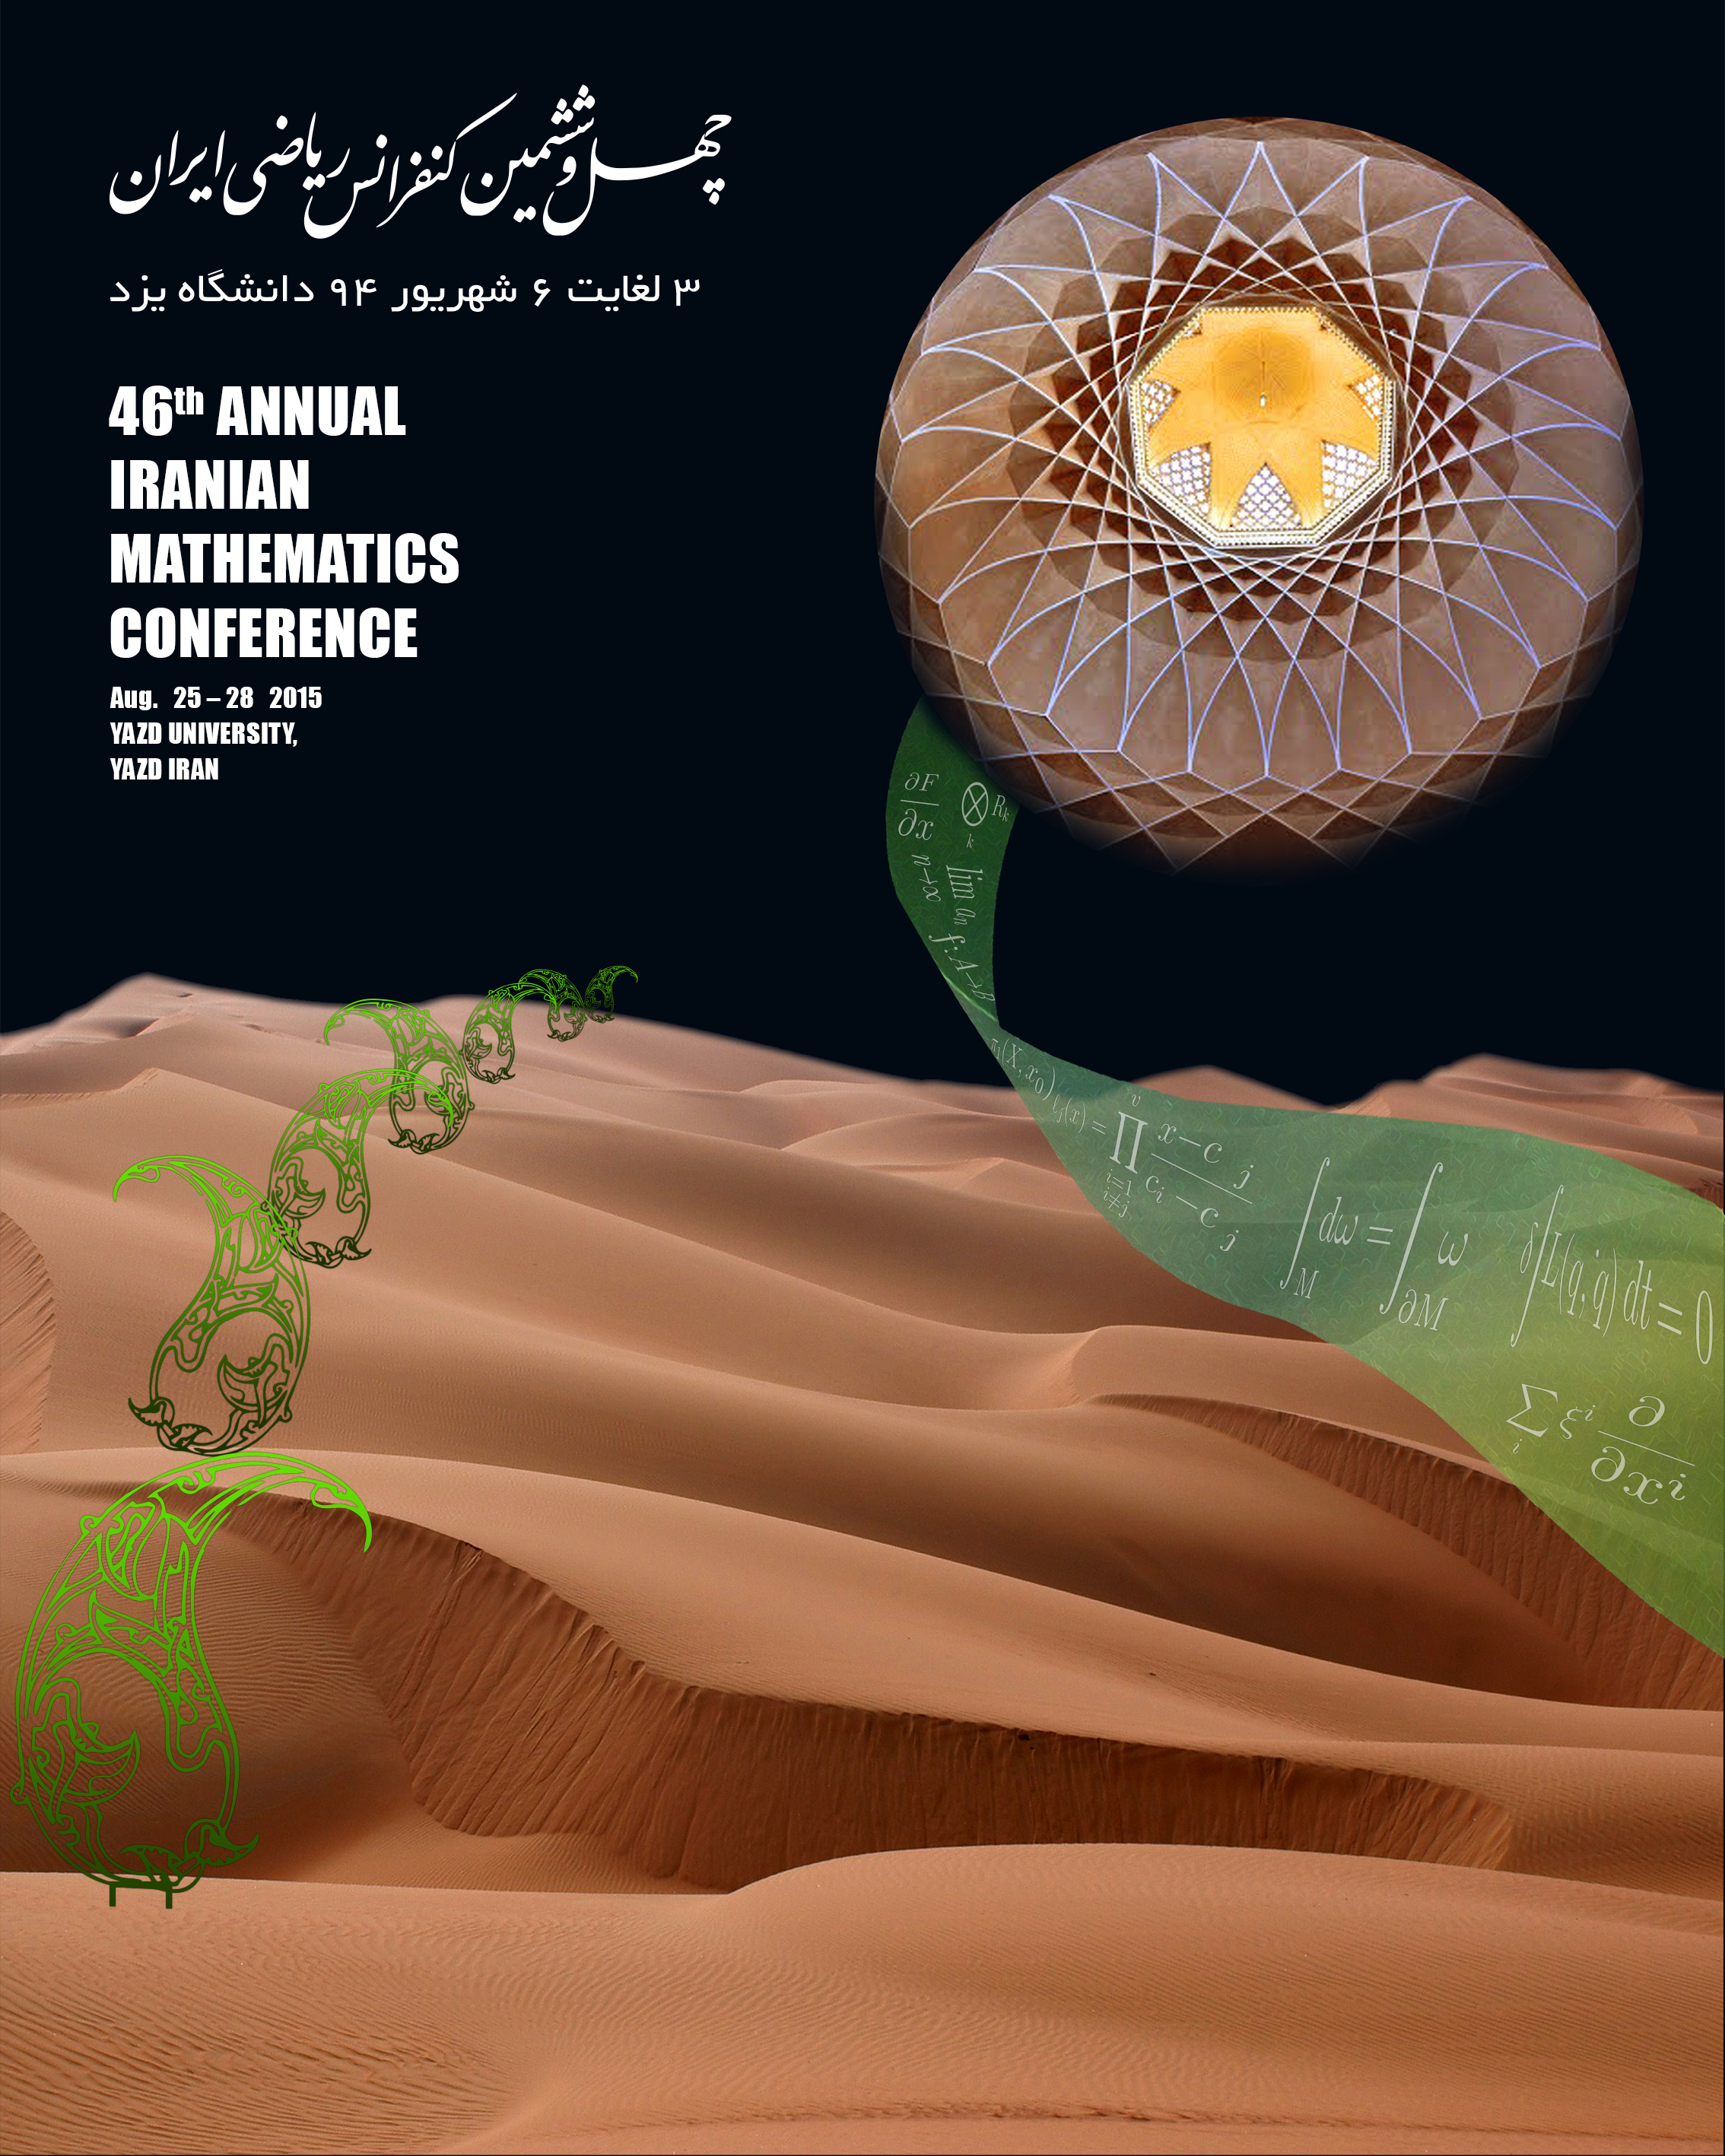
\includegraphics[width=\paperwidth,height=\paperheight]{poster.jpg}
  }%
}

\theoremstyle{definition}
\newtheorem{definition}{Definition}[section]
\theoremstyle{plain}
\newtheorem{theorem}[definition]{Theorem}
\newtheorem{lemma}[definition]{Lemma}
\newtheorem{proposition}[definition]{Proposition}
\newtheorem{corollary}[definition]{Corollary}
\theoremstyle{definition}
\newtheorem{example}[definition]{Example}
\newtheorem{remark}[definition]{Remark}
\newtheorem*{solution}{Solution}
\newcommand{\keywords}[1]{}
\newcommand{\subject}[1]{}

\begin{document}
 \BgThispage
\begin{center}
\veryHuge \color{NavyBlue} \textbf{A generalization of $\alpha$-dominating set and its complexity} \color{Black}\\ % Title
\huge \textbf{Davood Bakhshesh \& Mohammad Farshi \& Mahdieh Hasheminezhad}\\[0.5cm] % Author(s)
\huge Combinatorial and Geometric Algorithms Lab., Department of Computer Science\\ Yazd University, Yazd, Iran\\[0.4cm] % University/organization
\Large \texttt{{dbakhshesh@gmail.com},{mfarshi@yazd.ac.ir}, {hasheminezhad@yazd.ac.ir}
}--- 2333\\ % کد رهگیری مقاله
\end{center}
\vspace{1cm} % A bit of extra whitespace between the header and poster content

%----------------------------------------------------------------------------------------

\begin{multicols}{2} % This is how many columns your poster will be broken into, a portrait poster is generally split into 2 columns

%
\begin{abstract}\normalsize
Let $G=(V, E)$ be a simple and undirected  graph. For some real number $\alpha$ with $0<\alpha\leq1$, a set $D\subseteq V$ is called {an} {\it $\alpha$-dominating set} in  $G$ if every vertex $v$ outside $D$ has at least $\alpha\cdot d_v$ neighbor(s) in $S$ where $d_v$ is the degree of $v$. {The cardinality of a minimum $\alpha$-dominating set in a graph $G$ is called the} {\it $\alpha$-domination number} of $G$ and denoted by $\gamma_{\alpha}(G)$. In this paper, we introduce a generalization of $\alpha$-dominating set, that we call it {\it {\it $f_{deg}$-dominating} set}. Given a function $f_{deg}$ where $f_{deg}$ {is   as $f_{deg}:\mathbb{N}\rightarrow \mathbb{R}$} where $\mathbb{N}=\{1, 2, 3, \ldots\}$, and $f_{deg}$ may not be {an} integer-value function.  A set $D\subseteq V$ is called an  {$f_{deg}$-dominating} set in $G$ if for every vertex $v$ outside $D$, $|N(v)\cap D|\geq f_{deg}(d_v)$. In this paper, for this new concept, we will present some results on the its NP-completeness,  APX-completeness and  inapproximability. 
\end{abstract}
\keywords{Domination,  $\alpha$-Domination, $k$-Domination, APX-Complete, NP-Complete}
\subject{05C69, 11Y16}

\section{Introduction}
Let $G=(V, E)$ be an undirected and simple graph. A set $D\subseteq V$ is called {a} {\it dominating} set if every vertex  outside $D$ has at least one neighbor in $D$. {The} {cardinality} of a minimum dominating set is called {the} {\it domination number} of $G$ denoted by $\gamma(G)$.   In 2000,  Dunbar  et al.  \cite{dunbar2000alpha},  introduced the concept  of $\alpha$-domination. Let $\alpha$ be a real number with $0<\alpha\leq1$. A set $D\subseteq V$ is called an $\alpha$-dominating set in $G$ if for every vertex $v$ outside $D$, $|N(v)\cap D|\geq \alpha\times d_v$ where $N(v)$ is the set of all neighbors of $v$ in  $G$, and $d_v:=|N(v)|$ is the degree of $v$. Also, let $k$ be a real number with $k\geq 1$. A set $D\subseteq V$ is called a  {\it $k$-dominating} set in $G$ if for every vertex $v$ outside $D$, $|N(v)\cap D|\geq k$.

Now consider the definition of $\alpha$-dominating. One generalization of this concept is that instead of having at least $\alpha\times d_v$ neighbors in $D$ for each vertex $v\not \in D$, we have at least $f(d_v)$  neighbors in $D$, for some special function $f$. By selecting $f(x)=\alpha x$, the definition match the  $\alpha$-dominating.   It seems that this generalization is much near to the reality. Hence,   in this paper, we define the  {\it $f_{deg}$-dominating} set. Given a function $f_{deg}$ where $f_{deg}$ {is   as $f_{deg}:\mathbb{N}\rightarrow \mathbb{R}$} where $\mathbb{N}=\{1, 2, 3, \ldots\}$, and $f_{deg}$ may not be {an} integer-value function.  A set $D\subseteq V$ is called an  {$f_{deg}$-dominating} set in $G$ if for every vertex $v$ outside $D$, $|N(v)\cap D|\geq f_{deg}(d_v)$. In this paper, we consider the graphs with   no isolated vertices. We can easily extend the results for the graphs with isolated vertices. In this paper,  {we prove the NP-completeness of the following problem: given a graph $G$ and a positive integer $k$, decide whether $G$ has {an} $f_{deg}$-dominating set  $S$ with $|S|\leq k$.} Moreover,  we prove that the problem of finding a minimum  $f_{deg}$-dominating set when $f_{deg}(x)=k$ (in the other words, the $k$-dominating set) for any integer $k\geq 1$ is APX-complete (there is no PTAS).  Also, we present some inapproximability result for the problem of finding a minimum  $f_{deg}$-dominating set for constant function $f_{deg}(x)=k$. 
\section{NP-completeness  result}
In this section,  we will  prove that the problem of finding {the} $f_{deg}$-domination number of a graph is NP-complete, for every given function $f_{deg}$ with some special properties.  It is well known that the following decision problem, denoted by 3-REGULAR DOMINATION (3RDM), is NP-complete \cite{garey2002computers}: given a 3-regular graph $G =(V, E)$ {and} a positive integer $k$, does  $G$ has a dominating set $S$ with $|S|\leq k$?  Now,  consider the following decision problem, denoted by  $f$-DOMINATION ($f$DM): given a graph $G =(V, E)$ without isolated vertices {and a} positive integer $k$, does $G$ has an $f_{deg}$-dominating set $S$ with $|S|\leq k$?

 We will show that $f$DM is NP-complete for some special functions. We will extend  the proof of the result in which that $\alpha$-domination is NP-complete (see \cite{dunbar2000alpha}). 
\begin{theorem}.
If an increasing function $f_{deg}$ with domain $\mathbb{N}$ satisfies
\\ 
${\bf  a}.~ \forall x\in \mathbb{N},  0<f_{deg}(x)\leq x,$
\\
${\bf  b}.~ \exists x_0>0 \mbox{ such that }\forall x\geq x_0, ~x+1\geq f_{deg}(x+3).$
\\
${\bf  c}.~\mbox{For every two integers }$x$ \mbox{ and } $y$,  f_{deg}(y+x)\leq f_{deg}(y)+f_{deg}(x),$
\\
${\bf  d}. ~{\mbox {For a given~} } x\in\mathbb{N}, \mbox{ there is } y\in \mathbb{N}, \mbox{such that } y>x \mbox{ and } f_{deg}(y)\leq x,$
\\
then, the problem $f$DM is an NP-complete problem.
\label{thmNPf}
\end{theorem}
\begin{proof}[Sketch of Proof]
Let $f_{deg}$ be an arbitrary function that has the conditions of the theorem. We fix the function $f$. We can easily see that  $fDM\in NP$. Now, we proof the completeness.    We make a transformation from 3RDM to $f$DM.  Suppose that   $x$ is  the smallest  integer such that $(x+1)\geq f_{deg}(x +3)$,  and  $y$ is  the largest integer with $y>x$ and $x\geq f_{deg}(y)$. Consider the complete graph  $K_{y+1}$  and assume that $U=\{v_1, v_2, \ldots, v_x\}$ is {a subset of vertices of $K_{y+1}$ with $x$ elements}. We call the vertex set of $K_{y+1}$ by $W$. 

We transform a 3-regular graph $G$ to a graph denoted by $\hat{G}$ by  joining each vertex of  set $U$ to all vertices of $G$.   Assume that $S$ is a dominating set in $G$ such that  $|S|\leq k$. Consider {the} set $D = S \cup U$. Using the conditions {\bf b} and {\bf d}, it is easy to see that $D$ is an $f_{deg}$-dominating set in  $\hat{G}$ with $|D|\leq x+k$.

Now, we assume that $D$ is an $f_{deg}$-dominating set in  $\hat{G}$ with $|D|\leq x+k$. Among all $f_{deg}$-dominating set in $\hat{G}$ with $|D|\leq x+k$, we suppose that $D$ is {the} one {with} maximum $|D\cap U|$. Also, without loss of generality we can suppose that  there is  a vertex in $W-U$ that is outside  $D$. Using conditions {\bf a, b, c,} and {\bf d}, it is not  hard to prove that the set $D \cap V(G)$ is  a dominating set in $G$ with $|D \cap V(G)|\leq k$. Because 3RDM  is  NP-complete \cite{garey2002computers}, $f$DM is also NP-complete for the function $f$ that satisfies the conditions of Theorem \ref{thmNPf}.
\end{proof}
There are many functions that satisfy the conditions of Theorem \ref{thmNPf}, such as $\sqrt{x},~ \ln x$ and $\frac{x}{2}$.
\section{APX-completeness result}
In this section, we prove that  the problem of finding a minimum  $f_{deg}$-dominating set of a graph with maximum degree  $k+2$ and  $f_{deg}(x)=k$ for any $k\geq 1$ is APX-complete (there is no PTAS). We denote  the problem of finding a minimum $f_{deg}$-dominating set of a graph where  $f_{deg}(x)=k$ by {\textsc{ Min}} $k$-{\textsc {Dom Set}}, and when the problem is restricted to the graphs with maximum degree $k+2$, we call it {\textsc{ Min}} $k$-{\textsc {Dom Set}}-$(k+2)$. 

At first{,} we recall the $L$-reduction. 
\begin{definition}
\label{defdef}
($L$-reduction)\cite{ausiello}. Given two NP optimization problems $F$ and $G$ and a polynomial transformation $f$ from instances of $F$ to instances of $G$, we say
that $f$ is an $L$-reduction if there are {two} positive constants
$\alpha$ and $\beta$ such that for every instance $x$ of~$F$
\begin{enumerate}
\item $opt_G(f(x))\leq \alpha opt_F (x)$
\item for every feasible solution $y$ of $f(x)$ with objective value $m_G(f (x),y) = c_2$ we can, in polynomial time, find a solution $y'$ of $x$ with $m_F (f (x),y')=c_1$ such that $|opt_F (x)-c_1|\leq \beta|opt_G(f (x))-c_2|$.
\end{enumerate}
\end{definition}
{To prove that a problem $F$ is APX-complete, it is {sufficient} to prove that}  $F\in$APX and there is an $L$-reduction  from some APX-complete problem to  problem $F$.

\begin{theorem}[\cite{cicalese2013approximability}]
\label{thm1kapx}
For a graph $G$, {\sc Min} $k$-{\sc Dom Set } can be approximated in polynomial time by a factor of $\ln(2\Delta(G))+1$ where $\Delta(G)$ is the maximum degree of  $G$.
\end{theorem}
\begin{theorem}
\label{thmApxkdom}
{\textsc{ Min}} $k$-{\textsc {Dom Set}}-$(k+2)$ is {an} APX-complete {problem} for any $k\geq 1$.
\end{theorem}
\begin{proof}[Sketch of Proof]
 The case $k=1$  proved in \cite{alimonti1997hardness}. Consider $k>1$. Clearly, by Theorem \ref{thm1kapx},  if {the degree of vertices of the graph} is bounded by a constant then the approximation ratio is constant. Thus {the} problem {\sc Min} $k$-{\sc Dom Set}-$(k+2)$ is in APX. Suppose that $G=(V, E)$ is a  graph  of bounded degree 3. Construct a graph $G_k = (V_k, E_k)$ of bounded degree $k +2$ as follows.
Create a set $S_v$ of $k-1$ new vertices for each vertex $v$. Join each vertex $v \in V$ to $k-1$ vertices of $S_v$. Given a $k$-dominating set $D_k$ of $G_k=f_k(G)$ ({$f_k$ is a transformation from $G$ to $G_k$. Recall Definition} \ref{defdef}),  we can  find a dominating set $D$ in $G$ as $D=D_k-\left(\bigcup_{v\in V(G)}{S_v}\right)$. 
So  $\gamma(G)\leq |D|= |D_k|-(k-1)n$, where $n =|V|$. Also, given a dominating set $D$  of $G$, clearly  the set
$D_k=\left(\bigcup_{v\in V(G)}{S_v}\right)\cup D$
is a $k$-dominating set in $G_k$. So 
$\gamma_k(G_k)\leq |D_k|= |D|+(k-1)n$. Hence, we can easily conclude that $\gamma_k(G_k)=\gamma(G)+(k-1)n$.


Finally, using the above argument, we can find an  $L$-reduction with parameters  $\alpha=4k-3$ and $\beta=1$. So, the problem {\textsc{ Min}} $k$-{\textsc {Dom Set}}-$(k+2)$ is APX-complete. 
\end{proof}
\section{Inapproximability result on {\sc Min} $k$-{\sc Dom Set} }
In this section, we presents some inapproxmabillity result for {\sc Min} $k$-{\sc Dom Set}. 
\begin{theorem}[\cite{chlebik2008approximation}]
\label{thmepdom}
For any constant $\epsilon>0$ there is no polynomial time algorithm approximating {\sc Min 1-Dom Set} within a factor of $(1-\epsilon)\ln n$ unless NP $\subseteq$ DTIME($n^{O(\log \log n)}$). The same result {holds} for  bipartite graphs.
\end{theorem}
\begin{theorem}
For every $k \geq 1$ and every $\epsilon >0$, there is no polynomial time algorithm approximating {\.sc Min} $k$-{\sc Dom Set} for bipartite graphs within a factor of $(1-\epsilon) \ln n$, unless NP $\subseteq$ DTIME($n^{O(\log \log n)}$).
\end{theorem}
\begin{proof}[Sketch of Proof]
It is {sufficient} that, we make some modifications in the proof of Theorem \ref{thmepdom}. We make a reduction from domination on a bipartite graph $G$ with $n$ vertices such that $n+2k-2 \leq n^{1+\epsilon}$
and $\gamma(G).\geq \frac{2(k-1)(1+2\epsilon)}{\epsilon^2}.$ Then we transform the bipartite graph $G=(V_1,V_2, E)$ into a  bipartite graph $G'$ by adding to it two sets $K_1$ and $K_2$ each have $k-1$ new vertices inducing a graph {with} no edges.  Join each vertex of $V_1$ to each vertex of $K_2$ and join each vertex of $V_2$ to each vertex of $K_1$. We can easily prove that $\gamma_k(G')\leq \gamma(G)+2k-2$.
 Now,  suppose that there is a polynomial time approximation algorithm that computes a $k$-dominating set $D'$ for $G'$ such that  $|D'|\leq (1-\epsilon)\ln(|V(G')|)\gamma_k(G')$. It is easy t.o see that  $D:=D'\cap V(G)$ is a dominating set in  $G$. So, 
\begin{align*}
|D|&\leq|D'|\\
&\leq(1-\epsilon)(\ln |V(G')|) \gamma_{k}(G')~\mbox{(suppose that  $n:=|V(G')|$})\\
&\leq(1-\epsilon)(\ln n)  ({1+\epsilon+\epsilon^2})\gamma(G)\\
&=(1-\epsilon')(\ln n)\gamma(G),
\end{align*}.
where $\epsilon'=\epsilon^3>0.$  Therefore, the set $D$ approximates a minimum dominating set in  $G$  within factor $(1-\epsilon')\ln n$. But this contradicts Theorem \ref{thmepdom}. This completes the proof.
\end{proof}
\section{Figure and Table}
\begin{center}\vspace{1cm}
\includegraphics[width=0.5\linewidth]{example-image-a}
\captionof{figure}{\color{Green} A sample figure caption}
\label{vfig1}
\end{center}\vspace{1cm}


Here goes a table. Tables are ``float" objects.  It means that \LaTeX{} does not generally
place them on the same location in the source code as on the output. You can place them 
anywhere in the source code and then simply refer to them, like Table \ref{vtab1}.

\begin{center}\vspace{1cm}
\begin{tabular}{ccc}
\hline
First column head & Second column head & Third column head \\ \hline
N/A & $x^2+1$ & $6$ \\ 
$-20$ & $y$ & $11$ \\ 
$-12$ & $x+y$ & $7$\\
\hline
\end{tabular} 
\captionof{table}{\color{Green} A sample table caption}\label{vtab1}
\end{center}


\begin{thebibliography}{9}
\bibitem{alimonti1997hardness}
P.~Alimonti a.nd V.~Kann,
\newblock {\em Hardness of approximating problems on cubic graphs,}
\newblock Proceedings of the Third Italian Conference on Algorithms and Complexity, { Lecture Notes in Computer  Science}, pages 288--298, 1997.
\bibitem{ausiello}
G.~Ausiello,
\newblock {\em Complexity and approximation: Combinatorial optimization  problems and their appr.oximability properties,}
\newblock Springer Science Business Media, 1999.
\bibitem{chlebik2008approximation}
M.~Chleb{\'\i}k and J.~Chleb{\'\i}kov{\'a},
\newblock {\em Approximation hardness of dominating set problems in bounded degree
  graphs,}
\newblock {Information and Computation}, 206(11):1264--1275, 2008.
\bibitem{cical.ese2013approximability}
F.~Cicalese, M.~Milani{\v{c}}, and U.~Vaccaro,
\newblock {\em On the approximability and exact algorithms for vector domination and
  related problems in graphs,}
\newblock {Discrete Applied Mathematics}, 161(6):750--767, 2013.
\bibitem{dunbar2000alpha}
J.~E. Dunbar, D.~G. Hoffman, R.~C. Laskar, and L.~R. Markus,
\newblock {\em $\alpha$-domination,}
\newblock {Discrete mathematics}, 211(1):11--26, 2000.
\bibitem{garey2002computers}
M.~R. Garey and D.~S. Johnson,
\newblock {\em Computers and intractability: A Guide to the Theory of  NP-Completeness,}
\newblock Freeman, New York, 1979.
\end{thebibliography}

\end{multicols}
\end{document}
